% !TEX root = ../thesis.tex
\section{Equations}
	\label{sec:typesetting_equations}
	
Typesetting equations is one of the things that \LaTeX{} does best. It has packages for different fonts and symbols for many different mathematical notations.
However, to a person learning how to typeset in \LaTeX{} for the first time it can be a daunting and unwieldy user experience.
Almost all \LaTeX{} packages have documentation available in PDF format online, and documentation for packages specifically relating to fonts and symbols usually have tables enumerating the names and codes for all of the fonts symbols, organised by intended usage. 


	\subsection{Inline equations}

Small equations like \(x = 0\) can be written directly within the text by using \LaTeX{}'s maths mode shorthand controlled by parentheses: \lstinline|\(math mode\)| (preferred) or dollar signs: \lstinline|$math mode$|.
As long as it is does not become cumbersome to the reader, equations such as \(\mathbb{P}({A} \cap {B}) = \mathbb{P}({B} \cap {A})\) are quite neatly displayed in this fashion. 


	\subsection{Block equations}

For long equations it is best to provide a break in the main text of the document and format the equation using a \lstinline|\begin{equation}...\end{equation}| environment. 

		\begin{equation} \label{eq:veclen}
			\left\lvert a \right\rvert = \left\lvert \left[\begin{array}{c} a_0\\ a_1\\ \vdots\\ a_n\end{array}\right] \right\rvert = \sqrt{a_0^2 + a_1^2 + \hdots + a_n^2}
		\end{equation}
		
\Cref{eq:veclen} demonstrates formatting a larger equation and uses an \lstinline|\begin{array}...\end{array}| environment to structure a column vector of sub-equations.
Block equations should be located at a relevant point directly as they are being referred to in the text.
When referred to from other locations in the document you should use the \lstinline|\cref{key}| command to insert the correct equation number.


		\subsubsection{Aligning multi-line block equations}

When equations become even larger they may need cross over multiple new lines.
When this happens it is desirable to align relevant parts of the equation on each line to one another for aesthetic reasons and to help imply structure to the reader. 

			\begin{equation} \label{eq:rendering_equation}
				\begin{split}
					\mathcal{L}_o\left(x, \omega_o, \lambda, t\right) &= \mathcal{L}_e\left(x, \omega_o, \lambda, t\right)\\
					&+ \int_\Omega f\left(x, \omega_i, \omega_o, \lambda, t\right) \mathcal{L}_i\left(x, \omega_i, \lambda, t\right) \left(\omega_i \bullet n\right) d\omega_i\\
					&\text{where} \quad \mathcal{L}_i\left(x, \omega_i, \lambda, t\right) = \mathcal{L}_o\left(x^\prime, -\omega_i, \lambda, t\right)\\
				\end{split}
			\end{equation}

\Cref{eq:rendering_equation}, known as Kajiya's Rendering Equation \cite{kaj86} demonstrates the use of the \lstinline|\begin{split}...\end{split}| environment which uses a single un-escaped \& symbol placed on each line of the equation's \LaTeX{} code to indicate where each line should be co-aligned.
In this example the \&s were placed on the =, +, and w (in where) characters.


	\subsection{A masochistic approach to learning to typeset mathematics in \LaTeX{}}

		% !TEX root = ../thesis.tex
% [H] means put the figure HERE, directly when you input this code.
% Remove this to let LaTeX place the figure where it decides is best
\begin{figure}[H]
	\centering
	
% Note that we use the frame option to make latex put a 1 pixel black border 
% around the image. This is useful when the image has a white or transparent 
% background and will be displayed on white.
	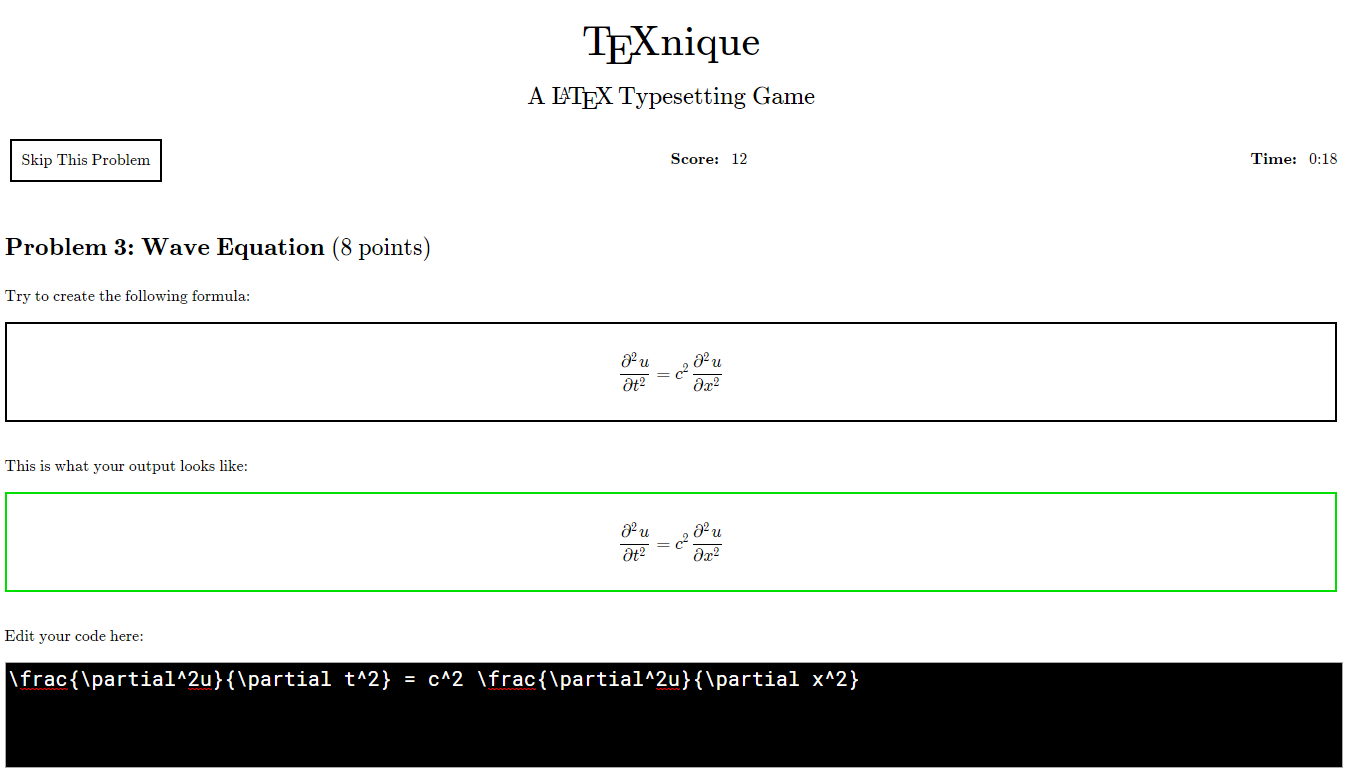
\includegraphics[width=1.0\textwidth,frame]{texnique.png}

% Caption is defined with a short and long version. The short version is shown in the 
% List of Figures section, and the long version is used directly with the figure. 			
	\caption[A screenshot of \TeX{}nique, a game about typesetting equations.]{
\TeX{}nique, a game about typesetting equations \cite{texnique}.
(Top) The game presents you with a rendered equation, (Bottom) the task is to enter \LaTeX{} code that produces the same rendered equation.
The green border on the lower rendering indicates it is a valid solution.
	
% Figure labels should be defined at the end of the caption to ensure proper numbering.
	\label{fig:texnique}
	}
\end{figure}

\TeX{}nique \cite{texnique} is web-browser based game for practising how to typeset equations in \LaTeX{}.
The game will present you with a rendered equation and your task is to type \LaTeX{} code into the box below it such that your code produces the same (or closely matching / pixel-equivalent) rendered equation.
\Cref{fig:texnique} shows the game during play~-- the bottom rendered equation is bordered in green to indicate it is a valid match with the target. 

		% An example of how to centre a passage of text, control local fontsize, 
		% and create a properly formatted and clickable URL.
		\begin{center}
		{\small \url{https://texnique.xyz}}
		\end{center}
		
This is one of the more painful parts of typesetting a document, so it really takes a special kind of sadism to come up with such a game.
Least to say, graduate students and researchers can be an odd bunch, and when we found this it was surprisingly addictive to compete over. 
